Um die Umsetzbarkeit diese Projektes zu überprüfen, wurde ein Prototyp angefertigt.

\section{Konstruktion}
Aus einem alten Schlauboot wurde der Boden ausgeschnitten. Danach wurde in einem Holzplatte in der Mitte ein Loch geschnitten und der Motor mit Propeller wurde darüber montiert -- siehe \autoref{fig:ErsterPrototyp}.
\begin{figure}[h!]
  \centering
  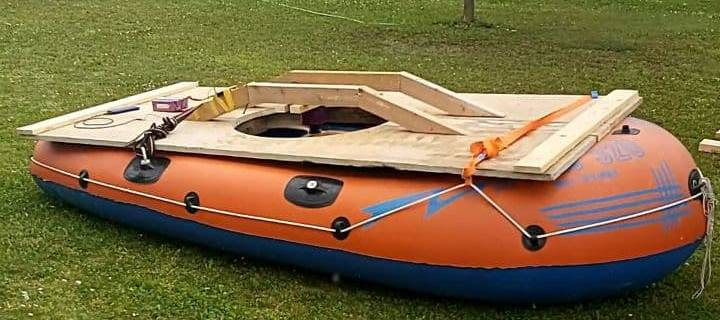
\includegraphics[width=.95\textwidth]{./Aufbau1.jpg}
  \caption{Aufbau erster Prototyp}
  \label{fig:ErsterPrototyp}
\end{figure}

Der Test war erfolgreich.
